\documentclass[conference]{IEEEtran}
\IEEEoverridecommandlockouts

\usepackage{cite}
\usepackage{amsmath,amssymb,amsfonts}
\usepackage{mathtools}
\usepackage{algorithmic}
\usepackage{graphicx}
\usepackage{subfigure}
\usepackage{textcomp}
\usepackage{xcolor}
\usepackage{textcomp}
\usepackage{float}
\usepackage{array}
\usepackage{siunitx}
\usepackage{tabularx}
\usepackage{listings}
\usepackage{accents}
\usepackage{nicematrix,tikz}
\usepackage{setspace}
\usepackage{xcolor}    % For text color
\usepackage{tcolorbox} % For colored boxes
\usepackage[colorlinks=false]{hyperref}
\def\BibTeX{{\rm B\kern-.05em{\sc i\kern-.025em b}\kern-.08em
    T\kern-.1667em\lower.7ex\hbox{E}\kern-.125emX}}

\setlength{\parindent}{0pt}

% Define the custom column type Y
\newcolumntype{Y}{>{\centering\arraybackslash} m{1cm}}

\definecolor{codeblue}{rgb}{0.2,0.2,0.6}
\definecolor{codegreen}{rgb}{0.133,0.545,0.133}
\definecolor{codegray}{rgb}{0.5,0.5,0.5}
\definecolor{codepurple}{rgb}{0.58,0,0.82}
\definecolor{backcolour}{rgb}{0.95,0.95,0.92}

\lstdefinestyle{mystyle}{
    backgroundcolor=\color{backcolour},
    commentstyle=\color{codegreen},
    keywordstyle=\color{codeblue},
    numberstyle=\tiny\color{codegray},
    stringstyle=\color{codepurple},
    basicstyle=\ttfamily\scriptsize,
    breakatwhitespace=false,
    breaklines=true,
    captionpos=b,
    keepspaces=true,
    numbers=none,
    numbersep=5pt,
    showspaces=false,
    showstringspaces=false,
    showtabs=false,
    tabsize=2
}
\lstset{style=mystyle}

% Define the custom style for error messages
\tcbuselibrary{listingsutf8}
\newtcblisting{terminalerror}{
  colframe=red!75!black, % Frame color
%   colback=red!10,        % Background color
  coltitle=red!75!black, % Title color
  fonttitle=\bfseries,   % Title font
  listing only,
  listing options={
    basicstyle=\footnotesize\ttfamily\color{red!75!black}, % Text style
    breaklines=true,       % Automatic line breaking
    escapeinside=``        % To escape to LaTeX
  },
%   title=Error Message,    % Box title
%   enhanced,               % Enable advanced features
%   attach boxed title to top left={
%     yshift=-2mm,           % Only yshift is needed here
%     xshift=2mm
%   },
%   boxed title style={
%     colframe=red!75!black,
%     colback=red!10,
%     sharp corners
%   },
  boxrule=0.2mm,          % Box border thickness
  left=1mm,               % Left padding
  right=1mm,              % Right padding
  top=-1mm,                % Top padding
  bottom=-1mm              % Bottom padding
}

% Define the custom style for error messages
% \newtcolorbox{terminalerror}{
%   colframe=red!75!black,    % Frame color
%   colback=red!10,           % Background color
%   coltitle=red!75!black,    % Title color
%   fonttitle=\bfseries,      % Title font
%   title=Error Message,      % Box title
%   fontupper=\footnotesize\ttfamily\color{red!75!black}, % Text style with footnotesize
%   boxrule=0.5mm,            % Box border thickness
%   left=2mm,                 % Left padding
%   right=2mm,                % Right padding
%   top=2mm,                  % Top padding
%   bottom=2mm,               % Bottom padding
% %   sharp corners,            % Sharp corners
%   colbacktitle=red!20,      % Background color of the title
%   coltitle=red!75!black,    % Title color
%   detach title,             % Detach title from box
%   before upper={\tcbtitle\par}, % Place title before the content
% }


% Define the custom inline error message style
\newcommand{\error}[1]{\textcolor{red!75!black}{\footnotesize \texttt{#1}}}
% Define the custom inline terminal input command style
\newcommand{\command}[1]{\textcolor{gray}{\footnotesize \texttt{#1}}}

\title{Robotics and Mechatronics\\
{\LARGE Mini Project Three}
}

\author{\IEEEauthorblockN{Mohammad Montazeri}
    \IEEEauthorblockA{\textit{School of Mechanical Engineering} \\
        \textit{College of Engineering, University of Tehran}\\
        Tehran, Iran; 810699269 \\
        mohammadmontazeri@ut.ac.ir}
}

\begin{document}
\maketitle

\begin{abstract}
    Robot Operating System (ROS) is a flexible framework for writing robot software, offering tools, libraries, and conventions to simplify the creation of complex and robust robot behavior. This project leverages \texttt{turtlesim}, a popular educational simulator within ROS, to develop practical expertise in ROS. The objective is to control, manipulate, and modify the \texttt{turtlesim} environment. Through these activities, the project aims to enhance users' proficiency in ROS, preparing them for more advanced robotic programming and development tasks.
\end{abstract}

\begin{IEEEkeywords}
    ROS, turtlesim, command, error, service
\end{IEEEkeywords}

\section{Introduction}
The Robot Operating System (ROS) is a powerful and versatile framework designed to simplify the development of robot software. It provides a rich set of tools, libraries, and conventions that enable the creation of complex and scalable robotic applications. One of the key educational tools within ROS is \texttt{turtlesim}, a simple yet effective simulator that allows users to control a virtual turtle within a graphical environment. By interacting with \texttt{turtlesim}, users can learn and practice essential ROS concepts such as topics, services, and parameters. This project aims to utilize \texttt{turtlesim} to gain hands-on experience in controlling and manipulating the simulation environment, thereby building a strong foundation in ROS that will be beneficial for more advanced robotic programming and development endeavors. The main objective is to draw the assigned characters shown in Figure~\ref{fig:chars} using turtles in \texttt{turtlesim} environment and then rotating them on their own coordinates. For a bonus point, both of these characters will be ready to move by the client's will, using keyboard arrow keys.

\begin{figure}[htbp]
    \centering
    \subfigure[Greek ``pi'' symbol]{
        
\includegraphics[width=0.19\textwidth]{figures/pi.png}
        % \label{fig:subfig1}    
    } \hfill
    \subfigure[English number ``five'' symbol]{
        
\includegraphics[width=0.2\textwidth]{figures/five.png}
        % \label{fig:subfig2}    
    }
    \caption{First (left \cite{b5}) and second (right) assigned characters for this project}
    \label{fig:chars}
\end{figure}

\section*{Services Available for \texttt{turtlesim} in ROS}
In the Robot Operating System (ROS), the \texttt{turtlesim} package is a popular tool used to teach and demonstrate various ROS concepts (Figure~\ref{fig:turtlesim}). First of all, we need to gain a better understanding of \texttt{turtlesim} and standard services available for it. Here is a thorough list of services you can see by executing \texttt{turtlesim\_node} and running \command{rosservice list}:

\subsection{\texttt{/clear}}
\begin{itemize}
    \item \textbf{Service Type}: \texttt{std\_srvs/Empty}
    \item \textbf{Description}: This service clears the turtlesim background, essentially removing any drawings made by the turtle. It resets the simulation background to the initial state without moving the turtle.
\end{itemize}

\subsection{\texttt{/kill}}
\begin{itemize}
    \item \textbf{Service Type}: \texttt{turtlesim/Kill}
    \item \textbf{Description}: This service deletes a turtle from the simulation. You need to provide the name of the turtle you want to remove.
    \item \textbf{Usage}: You call this service with the name of the turtle as a parameter.
\end{itemize}

\subsection{\texttt{/reset}}
\begin{itemize}
    \item \textbf{Service Type}: \texttt{std\_srvs/Empty}
    \item \textbf{Description}: This service resets the turtlesim to its original state, which includes clearing the background and resetting the position and orientation of the default turtle to its starting location.
\end{itemize}

\subsection{\texttt{/spawn}}
\begin{itemize}
    \item \textbf{Service Type}: \texttt{turtlesim/Spawn}
    \item \textbf{Description}: This service spawns a new turtle at a specified location and orientation. You need to provide the coordinates (x, y), the orientation (theta), and optionally the name for the new turtle.
    \item \textbf{Usage}: This is used when you want to add new turtles to the simulation.
\end{itemize}

\subsection{\texttt{/turtle1/set\_pen}}
\begin{itemize}
    \item \textbf{Service Type}: \texttt{turtlesim/SetPen}
    \item \textbf{Description}: This service changes the properties of the turtle's pen, such as color (r, g, b), width, and whether the pen is up or down (drawing or not drawing).
    \item \textbf{Usage}: Useful for changing the drawing style of the turtle.
\end{itemize}

\subsection{\texttt{/turtle1/teleport\_absolute}}
\begin{itemize}
    \item \textbf{Service Type}: \texttt{turtlesim/TeleportAbsolute}
    \item \textbf{Description}: This service teleports the turtle to an absolute position in the simulation with a specified orientation.
    \item \textbf{Usage}: This can be used to move the turtle instantly to any position within the simulation space.
\end{itemize}

\subsection{\texttt{/turtle1/teleport\_relative}}
\begin{itemize}
    \item \textbf{Service Type}: \texttt{turtlesim/TeleportRelative}
    \item \textbf{Description}: This service teleports the turtle relative to its current position and orientation.
    \item \textbf{Usage}: You can move the turtle forward by a specified distance and rotate it by a specified angle.
\end{itemize}

\subsection{\texttt{/turtle1}}
\begin{itemize}
    \item \textbf{Service Type}: \texttt{std\_srvs/Empty}
    \item \textbf{Description}: This is not actually a standard service but a node namespace prefix. By default, turtlesim starts with one turtle named ``turtle1''. Services related to this turtle will typically use this namespace.
\end{itemize}

\begin{figure}[htbp]
    \centerline{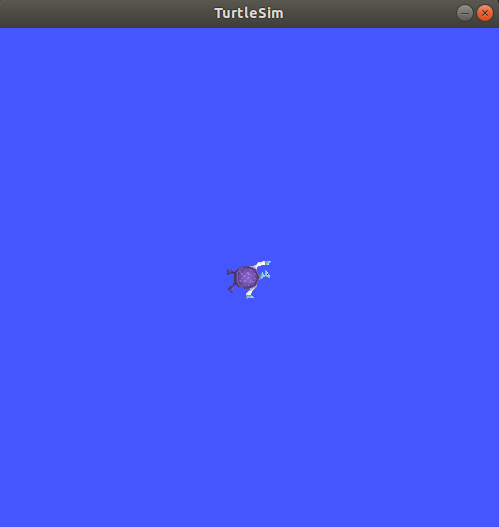
\includegraphics[width=0.34\textwidth]{figures/turtlesim.png}}
    \caption{A simple overview of turtlesim environment. \cite{b3}.}
    \label{fig:turtlesim}
\end{figure}
\vspace{10px}

These services allow us to manipulate the \texttt{turtlesim} environment in various ways, providing a comprehensive toolset for learning and demonstrating ROS functionalities. We will be using some of these features towards our own targets later.

\section{Workflow of the Program}
Here's the main sequence a client should traverse to get the desired response from the provided program.
\begin{enumerate}
    \item copy the \textit{catkin\_ws} appended to this report to your \textit{catkin} directory.
    \item source the files to acquaint the \textit{roscore} with the \textit{my\_pkg} package; this must be done using this bash command: \command{source ~/catkin\_ws/devel/setup.bash}
    \item specify which of the two characters shown in Figure~\ref{fig:cahrs} you want to be sketched on \textit{turtlesim} environment as you launch the files using this bash command: \command{roslaunch my\_pkg my\_launch.launch character:=1} \footnote{leaving the parameter empty will show the first character by default.}
    \item wait to see the turtles emerging on the screen gradually.
    \item enjoy the scenery for 1.2 seconds until the rotation of turtles start.
    \item click on the terminal and use arrow keys to move the turtles wherever you want; note that it's recommended to avoid colliding with walls which causes yellow warnings on tour terminal; it must also be noted that working with arrow-keys is a little bit tricky here, since there might be lags, unwanted movements, untracked key-presses and delays based on the processing capabilities of the your system's resources.\footnote{don't forget to select the terminal window before working with arrow-keys, and remember to hold the keys as long as it takes the turtles to respond.}
    \item exit the program using \underline{ctrl+c} in the running terminal window.
\end{enumerate}

\section{Investigation of Codes}
In this section, we'd have a brief explanation of the codes written for this project. Although all codes have sufficient comments which make them realizable, this section is suggested to be read for further information.
\subsection{Overview}
This report comes along a directory containing the \textit{catkin workspace} which includes the \textit{build}, \textit{devel} and \textit{src} folders. The \textit{build} directory contains files compiled with \command{catkin\_make} command; \textit{devel} directory also contains project files which are beyond the subject of this assignment. The \textit{src} folder, however, contains the base files of this project, under the package-name of \textit{my\_pkg}. Here's where one can see the \underline{script} files (\command{drawer.py}) in \textit{src} folder and \underline{launch} files (\command{my\_launch.launch}) in \textit{launch} folder.
\subsection{Launch File}
Within \command{my\_launch.launch}, one can see that an \command{arg} tag is used to define a parameter used inside the script file later, to specify which of the 2 assigned characters must be initialized. Then the main \command{turtlesim\_node} is defined and a \command{/clear} service is called on it to erase unwanted drawing on the \textit{turtlesim} environment. The script file is then added along with its parameter which would be equal to '1' by default, if not specified when calling the launch file.
\subsection{Script File}
\begin{itemize}
    \item Within \command{drawer.py}, an interpreter is allocated to the program first, followed by importing the necessary libraries and packages.
    \item \command{key\_mapping} dictionary is then introduced to map the pressed arrow keys to the directions to which they point, used later to move the turtles.
    \item \command{get\_key} is used to read the keys pressed in the terminal while the \textit{turtlesim} environment is running.
    \item \command{flush\_input} is used to erase the previously entered keys from memory, in order to prevent lags in executing the key tasks.
    \item \command{Change\_bg\_color} function sets a new color (defined in RGB format) to the background of the \textit{turtlesim} environment. By default it applies a yellow color but one can specify any desired color by giving its R-G-B factors to this function, later in the main part of the code. This function also deletes the default turtle which comes with the \command{turtlesim\_node} by default.
    \item  \command{Drawer} function gets the name of the character designated to be sketched and based on that, decides which function to be executed next. It also provides the name list of all turtles created. The \textit{delay} parameter defined in this function controls how fast the turtles must be created.
    \item \command{Turtle\_pixel\_one} or \command{\_two} are used to iteratively \command{/spawn} turtles, pixel by pixel on the \textit{turtlesim} board. To do so, the \textit{x, y, theta} and \textit{name} of each turtle is specified based on the chosen character and passed to the \command{spawn\_client} which was borrowed from \command{Drawer} function.
    \item \command{Move\_turtles} function is used for linear and angular velocity of turtles, taken as \textit{speed} and \textit{angular.z} relatively. In this function, a list is defined as \command{publishers} which will contain the \textit{velocity-message publisher} of each turtle. Another list called \command{monitor} is also defined which will contain an object of \textit{Turtle\_pose} class for each turtle, which will monitor its pose and do other stuff.\footnote{this class will be explained later on its own section} The variable \textit{rate} controls the speed of motion signals and is set to 5 Hz. Then using \command{while not rospy.is\_shutdown()} loop, the motion of turtles start, splitting a thread to listen to the keyboard and another one to publish the velocity message of each turtle. These velocity messages are of type \underline{Twist} imported from \command{geometry\_msgs.msg}. Within this vital loop, if the pressed keys read by \command{get\_key} function were one of the pre-defined keys in \command{key\_mapping} dictionary, the corresponding linear velocity would be assigned to all turtles, after their angular velocity being temporarily set to zero via \command{obj.set\_orientation()} line; otherwise, turtles would keep their angular velocity specified by \textit{angular.z} parameter.
    \item \command{Turtle\_pose} class gets the name of a turtle and defines a \underline{subscriber} of its \textit{Pose}, which is a message type from \command{turtlesim.msg} publisher. Using \command{callback} method the \textit{x, y} and \textit{theta} of turtle is saved as \command{self.pose} and returned to any applicant via \command{get\_theta} method. \command{set\_orientation} method uses the same route as \command{Move\_turtles} function to temporarily set the angular velocity of turtle to zero so that it can move in one of the \textit{rightward, leftward, downward} and \textit{upward} uninterruptedly. This method also uses \command{TeleportAbsolute} service to set the \textit{theta} parameter of the turtle to zero, so it faces right, otherwise, its local \textit{left, right, up} and \textit{down} directions would differ from the global observer of the \textit{turtlesim} board.
    \item In the main trunk of the program, its node would be initiated under the name \command{TurtleCharacter}.
    \item Using \command{rospy.get\_param}, the argument of the program which is the \textit{to-be-sketched character} is imported from the launch command.
    \item  Then the main functions explained above get called one by one to start the sequence of the program. Note that a slight delay of 1.2 seconds is put before rotating (and/or moving) the turtles so that the observer can thoroughly witness the sketched character before it starts shaking! By this, the codes end.
\end{itemize}
\vspace{20px}

\section{Errors and Handlings}
In this section, some of the errors occurred during the processes of working with ROS are mentioned and the solutions exerted to fix them are also briefly explained.

\subsection{Starting Turtlesim}
\label{sec:Starting_Turtlesim}
Error \error{[ERROR] [1717396146. 738976425]: [registerPublisher] Failed to contact master at [localhost: 11311]. Retrying ...} happened while trying to start up the turtlesim environment using \command{rosrun turtlesim turtlesim\_node} command. Turns out I hadn't have initialized ROS using \command{roscore} command.
\vspace{10px}

\subsection{Compiling packages after creating message file}
\label{sec:Compiling_packages}
The following error happened while trying to compile the entire \textit{catkin} workspace using \command{catkin\_make} after creating a new message file and modifying relevant files. Turns out I deleted the \command{FILES} line from the \textit{CMakeLists.txt} file. Re-adding that, solved the issue.
\begin{terminalerror}
    CMake Error at /opt/ros/noetic/share/genmsg/cmake/genmsg-extras.cmake:77 (message):
    add_message_files() called with unused arguments: demo_msg.msg
    Call Stack (most recent call first):
    demo_pkg/CMakeLists.txt:50 (add_message_files)
    Configuring incomplete, errors occurred!
    --
    See also "/home/saeed/catkin_ws/build/CMakeFiles/CMakeOutput. log".
    See also "/home/saeed/catkin_ws/build/CMakeFiles/CMakeError.log".
    Invoking "cmake" failed
\end{terminalerror}
\vspace{10px}

\subsection{Using \textit{Enter} instead of \textit{Tab}}
\label{sec:Using_Enter}
After creating a service of my own, consisting of a new `\textit{.srv}' file, a server and a client, I tried to run the server alone to see if it worked correctly. After using \command{rosservice list} to see my custom service name, \textit{meaner}, and advancing to give the arguments to \command{rosservice call /meaner}, I faced the error \error{Usage: rosservice call /service [args ... ]
rosservice: error: Please specify service arguments}. Turns out I had to use \textit{Tab} key after the mentioned command, instead of \textit{Enter}, which was the key I used.
\vspace{10px}


\subsection{Simultaneous launch despite system delay}
\label{sec:Simultanous_launch}
I struggled so much on running a trial launch file, which called the \command{/clear} service after it started the \command{turtlesim\_node}. It always got an error like \error{ERROR: Service [/clear] is not available.
        [clear-3] process has died [pid 3416, exit code 2, ...]}. That took a lot of my time to be debugged. I first thought that the problem came from my launch file and it needed to be compiled first. So I changed to the \command{~/catkin\_ws/} directory and tried to compile my package with \command{catkin\_make}. That caused a new error which I managed to solve eventually\footnote{This error is explained at section \ref{sec:Compile_error}.}, but didn't work out for the main error I used to get. So I kept manipulating my launch file, to get another error: Nodes with the same \textit{name} attribute\footnote{This error is explained at section \ref{sec:Nodes_with}}. Fixing that and keeping the same procedure to alter my launch file, I started to suspect that the \command{/clear} service comes from \command{std\_srvs}, not \command{rosservice}. Changing that in my launch file caused a new error which took me a lot of time and effort to fix\footnote{This error is explained at section \ref{sec:Incorrect_pkg}}. So starting back from the first steps, I tried to replace \command{/clear} service with other services defined for \command{turtlesim\_node} like \command{/kill}, \command{/reset} or \command{/spawn}. All of them confronted errors such as \error{ERROR: Service [/kill] is not available}. After that, sick of all my indecisive attempts, I took a long break to come back with a new idea from my web-searches: to execute my node as a bash-script. Although I was able to access my desired services (like \command{/clear}) in my python-scripts, but this idea was more mesmerizing. So I used the codes provided by AI \cite{b2} to create a node based on a new bash-script. That, too, got an error\footnote{This error is explained at section \ref{sec:Oblivion_of}}. Fixing that, I came to a relief when I saw my files launch uninterruptedly. Finally, turns out the nodes introduced in my launch file used to get executed so fast, that their order was not observed. In other words, the error I was encountering \error{ERROR: service [/clear] is not available} occurred because the turtlesim\_node might not have be fully initialized when the rosservice call was made. This could happen because the launch file started both nodes simultaneously without ensuring that the turtlesim\_node was fully ready. One way to ensure proper synchronization was to use the rosservice command with a slight delay to allow the turtlesim\_node to initialize properly. However, ROS launch files did not natively support delays directly. Instead, I used a small workaround by calling rosservice within a rosrun command with a shell script to introduce a delay. That's how this enormous and crucial error was resolved.
\vspace{10px}

\subsection{Compile error}
\label{sec:Compile_error}
As explained above, when I tried to compile my package with \command{catkin\_make}, I got \error{The build space at '/home/saeed/catkin\_ws/build' was previously built by ''. Please remove the build space or pick a different build space}. To fix that, I manually deleted the \textit{build} directory of my \command{~/catkin\_ws/} and retied the compile process.
\vspace{10px}


\subsection{Nodes with the same \textit{name} attribute}
\label{sec:Nodes_with}
Error \error{RLException: roslaunch file contains multiple nodes named [/TurtleCharacter].
    Please check all <node> 'name' attributes to make sure they are unique.} appeared when I executed one of my trial launch files, which contained two nodes, including \command{name="TurtleCharacter"}. Turns out nodal names must be unique.
\vspace{10px}


\subsection{Incorrect \textit{pkg} and \textit{type} attributes}
\label{sec:Incorrect_pkg}
When I used a node like \command{<node pkg="std\_srvs" type="Empty" name="turtle2" args="call /clear" />} within my launch file, I faced an error like \error{ERROR: cannot launch node of type [std\_srvs/Empty]: Cannot locate node of type [Empty] in package [std\_srvs]. Make sure file exists in package path and permission is set to executable (chmod +x)}. Turns out, unlike my temporary suspicion, the \command{/clear} command shouldn't be written as a launch node in this way; rather, it should be like: \command{<node pkg="rosservice" type="rosservice" name="clear" args="call /clear" />}.
\vspace{10px}


\subsection{Oblivion of permissions}
\label{sec:Oblivion_of}
I wrote my bash-script named \command{spawn\_turtle.sh} in the \command{src/} directory of my package, containing \command{sleep 5
    rosservice call /spawn 2 2 0.5 turtle2}. Then I added a node as \command{<node name="spawn\_turtle" pkg="my\_pkg" type="spawn\_turtle.sh" output="screen" cwd="node"/>} to my launch file. Launching this file faced \error{ERROR: cannot launch node of type [my\_pkg/spawn\_turtle.sh]: Cannot locate node of type [spawn\_turtle.sh] in package [my\_pkg]. Make sure file exists in package path and permission is set to executable (chmod +x)}. Turns out I hadn't have given the execution permission to the bash-script before using it in my launch file.
\vspace{10px}


\subsection{Connection error in Linux}
\label{sec:Connection_error}
Once I tried to start Linux on my virtual machine, when I confronted \error{*ERROR* Failed to send host log message.
        [FAILED] Failed to start Network Name Resolution.} Although I knew having my VPN turned on in my host OS (Windows) interrupts connection on Linux, this error got me surprized since my VPN was off. After a few times of rebooting the virtual box, and getting the same error, I figured out that my DNS address doesn't cope with the guest OS (Linux). I remembered that I had modified my DNS long ago to be able to bypass the OpenAI \cite{b2} sanctions on Iran DNS addresses. Resetting my IP and DNS solved the problem in the end.
\vspace{10px}


\subsection{Linux fatal error}
\label{sec:Linux_fatal}
I have been working couple of days on this project, using Oracle VM to bring up my Linux. Sometimes I left my system on sleep for many hours so it would automatically hibernate with the virtual box being opened. This, I believe, harmed my system gradually until I once confronted a blank dark screen in my Linux which didn't have any functionality. I restarted the VM or my entire PC for many times, but it didn't work. I believe the lack of memory space had to do something with it too, so I tried entering the bios environment to solve the problem. Despite all of my attempts to repair the system, even with following all of the instructions taken from the web, I wasn't able to rehabilitate the system. I even couldn't restore my files, which took a lot of my time and power to reach to a noticeable level. Frustrated and hopeless, I uninstalled the entire virtual machine and migrated to the online simulator introduced in the classroom, \textit{the Construct} \cite{b4}. Moving to this new environment, I had to start from scratch. That made me reconsider some of the previously mentioned error handlings. For example, I figured out that the resources this website allocates to me, in contrast to my own system, handles the ROS nodes better and faster. Thus the problem discussed in \ref{sec:Simultanous_launch} didn't ever happen in \textit{the Construct}. That's why I haven't included the mentioned bash script file in my project.
\vspace{10px}

\section{Conclusion}
\textbf{In this project, we successfully demonstrated the ability to manipulate and control the turtlesim simulation environment in ROS using Python. Our key accomplishments included \textit{Interactive Control} and \textit{Practical Application of ROS Tools}. Overall, this project provided a hands-on opportunity to explore the capabilities of ROS in a simulated environment, demonstrating how Python scripts can be used to control and modify simulations in real-time, thereby laying a foundation for more complex robotic applications and system integrations.}
\vspace{10px}

\section{Results}
Some videos from the workflow of this project are appended in this \href{https://drive.google.com/drive/folders/1shN1r_mjPmyW_KCoqPHrUwNnDsbRPgS5?usp=sharing}{link} along with supporting materials.

\begin{figure}[htbp]
    \centering
    \subfigure[Sketched character 2: ``pi'' symbol]{
        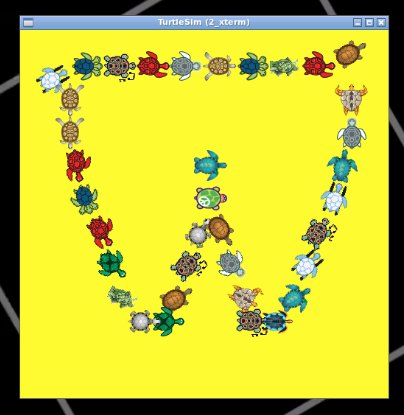
\includegraphics[width=0.4\textwidth]{figures/my_Pi.png}
        % \label{fig:subfig1}    
    }
    \subfigure[Sketched character 2: ``five'' symbol]{
        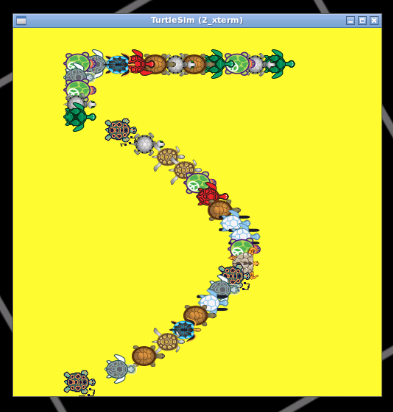
\includegraphics[width=0.4\textwidth]{figures/my_Five.png}
        % \label{fig:subfig2}    
    }
    \caption{Results for first (left) and second (right) assigned characters for this project}
    \label{fig:char_results}
\end{figure}


\begin{figure}[htbp]
    \centering
    \subfigure[Nodes only mode]{
        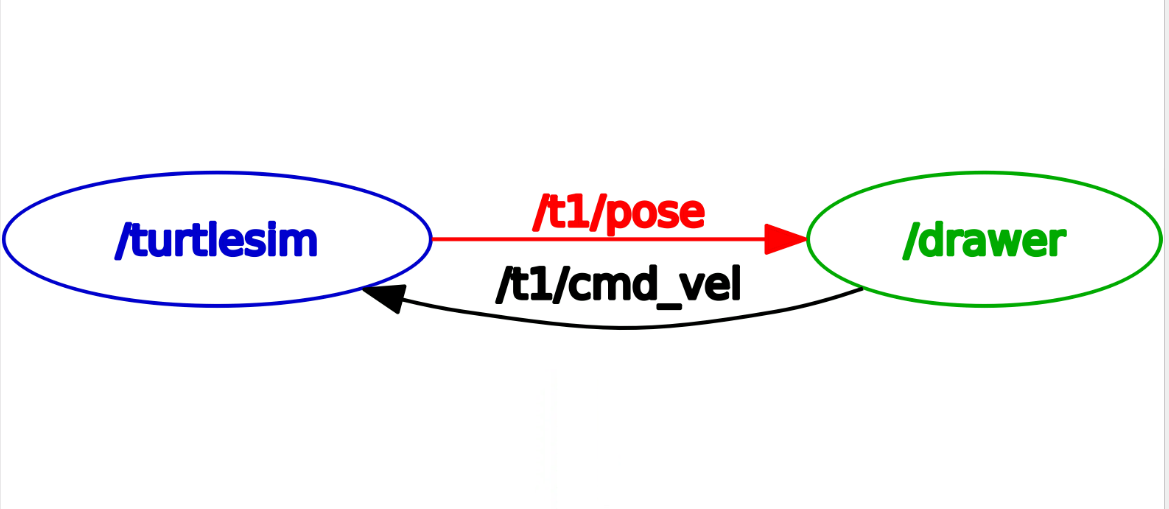
\includegraphics[width=0.4\textwidth]{figures/nodes_only.png}
        % \label{fig:subfig1}    
    } \vfill
    \subfigure[Nodes and Topics mode (partial view)]{
        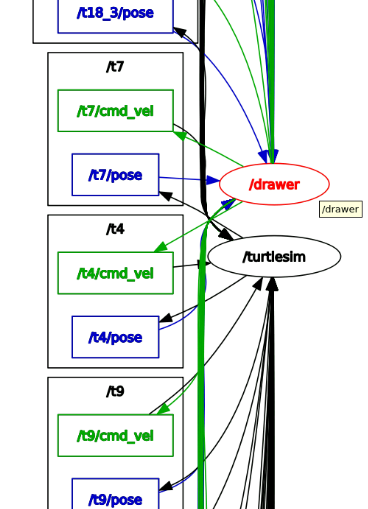
\includegraphics[width=0.4\textwidth]{figures/nodes_topics.png}
        % \label{fig:subfig2}    
    }
    \caption{Results from \command{rqt\_graph} for active nodes and topics overview}
    \label{fig:graph_results}
\end{figure}
\vspace{30px}


\begin{thebibliography}{00}
    \bibitem{b1} Open Robotics, ``Wiki ROS'', \url{https://wiki.ros.org/}

    \bibitem{b2} OpenAI, (2023), ChatGPT (Sep 25 version) [Large language model], \url{https://chat.openai.com/chat}

    \bibitem{b3} ROS Documentation, \url{https://docs.ros.org/en/foxy/Tutorials/Beginner-CLI-Tools/Introducing-Turtlesim/Introducing-Turtlesim.html}

    \bibitem{b4} The Construct: Where Your Robotics Career Happens, 2024, \url{https://app.theconstruct.ai/}

    \bibitem{b5} Image courtesy of \url{https://codepoints.net/U+03D6?lang=en} and \url{https://graphemica.com/%CF%96} 
\end{thebibliography}


\end{document}
